\documentclass[oneside, 11pt]{article}

\usepackage[T1]{fontenc}
\usepackage[utf8]{inputenc}
\usepackage[dutch]{babel}

\usepackage{fouriernc}
\usepackage[detect-all, load-configurations=binary,
            separate-uncertainty=true, per-mode=symbol,
            retain-explicit-plus, range-phrase={ tot }]{siunitx}

\usepackage{setspace}
\setstretch{1.2}

\setlength{\parskip}{\smallskipamount}
\setlength{\parindent}{0pt}

\usepackage{geometry}
\geometry{marginparwidth=0.5cm, verbose, a4paper, tmargin=3cm, bmargin=3cm, lmargin=2cm, rmargin=2cm}

\usepackage{float}

\usepackage[fleqn]{amsmath}
\numberwithin{equation}{section}
\numberwithin{figure}{section}

\usepackage{graphicx}
\graphicspath{{Figures/}}
\usepackage{subfig}

\usepackage{tikz}
\usetikzlibrary{plotmarks}

\usepackage{fancyhdr}
\pagestyle{fancy}
\fancyhf{}
\rhead{\thepage}
\renewcommand{\footrulewidth}{0pt}
\renewcommand{\headrulewidth}{0pt}

\usepackage{relsize}
\usepackage{xspace}
\usepackage{url}

\newcommand{\figref}[1]{Figuur~\ref{#1}}

\newcommand{\hisparc}{\textsmaller{HiSPARC}\xspace}
\newcommand{\kascade}{\textsmaller{KASCADE}\xspace}
\newcommand{\sapphire}{\textsmaller{SAPPHiRE}\xspace}
\newcommand{\jsparc}{\textsmaller{jSparc}\xspace}
\newcommand{\hdf}{\textsmaller{HDF5}\xspace}
\newcommand{\aires}{\textsmaller{AIRES}\xspace}
\newcommand{\csv}{\textsmaller{CSV}\xspace}
\newcommand{\python}{\textsmaller{PYTHON}\xspace}
\newcommand{\corsika}{\textsmaller{CORSIKA}\xspace}
\newcommand{\labview}{\textsmaller{LabVIEW}\xspace}
\newcommand{\daq}{\textsmaller{DAQ}\xspace}
\newcommand{\adc}{\textsmaller{ADC}\xspace}
\newcommand{\adcs}{\textsmaller{ADC}s\xspace}
\newcommand{\Adcs}{A\textsmaller{DC}s\xspace}
\newcommand{\hi}{\textsc{h i}\xspace}
\newcommand{\hii}{\textsc{h ii}\xspace}
\newcommand{\mip}{\textsmaller{MIP}\xspace}
\newcommand{\hisparcii}{\textsmaller{HiSPARC II}\xspace}
\newcommand{\hisparciii}{\textsmaller{HiSPARC III}\xspace}
\newcommand{\pmt}{\textsmaller{PMT}\xspace}
\newcommand{\pmts}{\textsmaller{PMT}s\xspace}

\DeclareSIUnit{\electronvolt}{\ensuremath{\mathrm{e\!\!\:V}}}

\DeclareSIUnit{\unitsigma}{\ensuremath{\sigma}}
\DeclareSIUnit{\mip}{\textsmaller{MIP}}
\DeclareSIUnit{\adc}{\textsmaller{ADC}}

\DeclareSIUnit{\gauss}{G}
\DeclareSIUnit{\parsec}{pc}
\DeclareSIUnit{\year}{yr}



\title{Cosmic air showers}
\author{J.M.C. Montanus}
\docalgemeen{2}{CS}
\version{1.0}

\begin{document}

\maketitle

\section{Kosmische deeltjes}

De aarde wordt continu `gebombardeerd' door deeltjes vanuit de ruimte.
Als zo'n deeltje de dampkring binnendringt zal het op een gegeven moment
een botsing maken met een luchtmolecuul. Met `botsing' bedoelen we niet
een botsing zoals tussen biljartballen. Bij een botsing tussen
biljartballen verandert wel de richting en snelheid van de
biljartballen, maar er ontstaan geen nieuwe biljartballen. Het is beter
te spreken van een \emph{wisselwerking} tussen het kosmisch deeltje en
een luchtmolecuul omdat tijdens de wisselwerking nieuwe deeltjes
ontstaan. Deze deeltjes zullen op hun beurt ook weer wisselwerken met
luchtmoleculen waardoor er nog meer nieuwe deeltjes ontstaan. Er
ontstaat als het ware een `lawine' van deeltjes, die in de
wetenschappelijke literatuur wordt aangeduid als \emph{cosmic air
shower}. Bij elke wisselwerking wordt de energie verdeeld over de nieuwe
deeltjes waardoor de energie per deeltje afneemt. Deeltjes waarvan de
energie te klein is om bij een wisselwerking nieuwe deeltjes te maken
dragen niet meer bij aan de ontwikkeling van de lawine; de lawine
`sterft uit'. Hoe groter de energie van het deeltje dat uit de ruimte
kwam, des te langer het duurt voor dat de lawine is uitgestorven. Als de
energie groot genoeg is kan de lawine het aardoppervlak bereiken. 

Van de deeltjes die in onze dampkring terechtkomen is een deel afkomstig
van de zon. De energie van deeltjes van de zon is betrekkelijk laag; ze
veroorzaken maar kleine lawines die al hoog in de atmosfeer zijn
uitgestorven. Soms zijn er op de zon wel eens uitbarstingen van grote
hoeveelheden geladen deeltjes. Deze kunnen in onze atmosfeer het
\emph{poollicht} of \emph{noorderlicht} veroorzaken
(\figref{fig:poollicht}). Dat we het poollicht kunnnen waarnemen komt
omdat er tijdens zo'n uitbarsting van de zon zeer veel deeltjes in onze
atmosfeer terechtkomen.

\begin{figure}
    \centering
    
\includegraphics[width=.7\textwidth]{poollicht_alaska.jpg}
    \caption{Poollicht boven Alaska \cite{strang}.}
    \label{fig:poollicht}
\end{figure}

Van verder weg uit de ruimte komen deeltjes met hogere energie. Van de
lawines die daaruit in onze atmosfeer ontstaan kunnen deeltjes het
aardoppervlak bereiken en een signaal afgeven in een \hisparc detector.
Op deze wijze kunnen we kosmische deeltjes indirect waarnemen. In deze
lesbrief zal worden ingegaan op de ontwikkeling van de shower in de
atmosfeer en de deeltjes die daarbij een belangrijke rol spelen. Eerst
gaan we kijken naar de eenheden waarin we de energie van een deeltje
kunnen uitdrukken. 


\section{De energie van een deeltje}

Volgens het SI eenhedenstelsel is de joule (J) de eenheid van energie
($\SI{1}{\joule} = \SI{1}{\kilo\gram\square\meter\square\second}$). In
de deeltjesfysica is dat geen handige eenheid. Van zowel elementaire
deeltjes als elektronen en muonen als samengestelde deeltjes als pionen
(opgebouwd uit 2 quarks) en protonen (opgebouwd uit 3 quarks) wordt de
energie vrijwel altijd uitgedrukt in elektronvolt
(\SI{}{\electronvolt}). Eén elektronvolt is de energieverandering van
een elektron als het een potentiaalverschil van \SI{1}{\volt} overbrugt.
Een elektronvolt is een zeer kleine hoeveelheid energie:
$\SI{1}{\electronvolt} = \SI{1,60e-19}{\joule}$. Om enig gevoel voor
dergelijke kleine energieën te krijgen bekijken we eens de energie van
een muon in rust. Deze is $E_0 = \SI{105,6}{\mega\electronvolt}$. Voor
een deeltje dat beweegt met snelheid $v$ is de energie groter:
\begin{equation}
    E(v) = \frac{E_0}{\sqrt{1-\frac{v^2}{c^2}}} \ . \nonumber
\end{equation}

Hierin is $c$ de lichtsnelheid. Als een muon een snelheid heeft dat
99,9\% is van de lichtsnelheid, dan is zijn energie 
\begin{equation}
    E(0,999c) = \frac{105,6}{\sqrt{1-0,999^2}}\SI{}{\mega\electronvolt}
    = \SI{2,36}{\giga\electronvolt}. \nonumber
\end{equation}

Uitgedrukt in joule zou deze energie een klein getal zijn. De waarde
\SI{2,36}{\giga\electronvolt} doet meer recht aan het feit dat de
energie relatief hoog is voor een elementair deeltje als het muon. 
\\

Kosmische deeltjes kunnen een relatief hoge energie hebben, tot wel meer
dan \SI{e20}{\electronvolt}. De energie van energetische deeltjes wordt
vaak uitgedrukt in \SI{}{\tera\electronvolt}, \SI{}{\peta\electronvolt},
etc. De betekenis daarvan staat in Tabel \ref{eenheden}.

\begin{table}[h]
    \centering
    \begin{tabular}{|c|l|r|} \hline
        factor & eenheid & symbool \\ \hline
        $10^0$ & elektronvolt & eV \\
        $10^3$ & kiloelektronvolt & keV \\
        $10^6$ & megaelektronvolt & MeV \\
        $10^9$ & gigaelektronvolt & GeV \\
        $10^{12}$ & teraelektronvolt & TeV \\
        $10^{15}$ & petaelektronvolt & PeV \\
        $10^{18}$ & exaelektronvolt & EeV \\
        $10^{21}$ & zettaelektronvolt & ZeV \\ \hline
    \end{tabular}
    \caption{Energie eenheden van deeltjes.}
    \label{eenheden}
\end{table}


\section{Showers}

Ruwweg kan er onderscheid gemaakt worden tussen twee soorten showers:
elektromagnetische showers en hadronische showers. Omdat de
elektromagnetische shower het eenvoudigst kan worden beschreven, zullen
we die het eerst behandelen. 


\subsection{Elektromagnetische showers}

Wanneer een kosmisch gamma-deeltje $\gamma$ (een hoogenergetisch foton)
de dampkring binnenkomt, kan het door elektromagnetische wisselwerking
met de kern van een luchtatoom opsplisten in een elektron $e^-$ en een
positron $e^+$. Dit proces heet paar-creatie. Wat verderop in de
dampkring kan het elektron vervolgens door elektromagnetische
wisselwerking met de kern van een luchtatoom een gamma-deeltje afstaan.
Hetzelfde geldt voor het positron. Dit proces heet remstraling. Weer wat
verderop in de dampkring zal er weer paar-creatie optreden bij de
gamma-deeltjes en remstraling bij de elektronen en positronen. Er komen
dus steeds meer deeltjes, maar die hebben elk wel een steeds kleinere
energie. Na een aantal splitsingen is de energie van een deeltje zo
klein dat het gemakkelijk zijn energie kwijtraakt aan het ioniseren van
een luchtatoom. Dat gebeurt als de energie van een deeltje nog maar zo'n
\SI{84}{\mega\electronvolt} is. Voordat het zover is kunnen er uit één
kosmisch deeltje een lawine van vele miljoenen deeltjes in de dampkring
ontstaan: de \emph{cosmic air shower} of kortweg \emph{shower}. Omdat
zowel paar-creatie als remstraling elektromagnetische processen zijn
spreekt men van een elektromagnetische shower. \\

Samenvattend wordt de elektromagnetische shower gedomineerd door paar-creatie
\begin{equation}
    \gamma \rightarrow e^- + e^+ \nonumber
\end{equation}
en remstraling
\begin{equation} 
    e^\pm \rightarrow e^\pm + \gamma \ . \nonumber
\end{equation}
In beide gevallen is er een `splitsing' van één deeltje in twee deeltjes.  


\subsection{Eenvoudig model voor de elektromagnetische shower}

Een eenvoudig model voor de ontwikkeling van het aantal deeltjes in een
elektromagnetische shower is het Heitler model. Volgens dit model
ondergaan de deeltjes die op een bepaald moment in de shower zitten
gelijktijdig een opsplitsing waarbij de energie van een deeltje gelijk
verdeeld wordt over de twee ontstane deeltjes. We noemen die
gemeenschappelijke opsplitsing een `stap'. Dus als we beginnen met een
deeltje met een energie van bijvoorbeeld \SI{8}{\peta\electronvolt}, dan
hebben we na de eerste stap 2 deeltjes van elk
\SI{4}{\peta\electronvolt}, na twee stappen 4 deeltjes van
\SI{2}{\peta\electronvolt}, na 3 stappen 8 deeltjes van
\SI{1}{\peta\electronvolt}, enzovoort. Na 27 stappen is de energie
minder dan \SI{84}{\mega\electronvolt} zodat de shower, volgens dit
model, stopt. Zolang de energie boven de stopenergie van
\SI{84}{\mega\electronvolt} zit groeit het aantal deeltjes volgens het
Heitler model exponentieel als functie van het aantal stappen om
vervolgens plotseling op te houden. Als de begin energie
\SI{8}{\peta\electronvolt} is, gebeurt dat op circa \SI{3}{\km} hoogte
(\figref{fig:heitler}). 

\begin{figure}
    \centering
    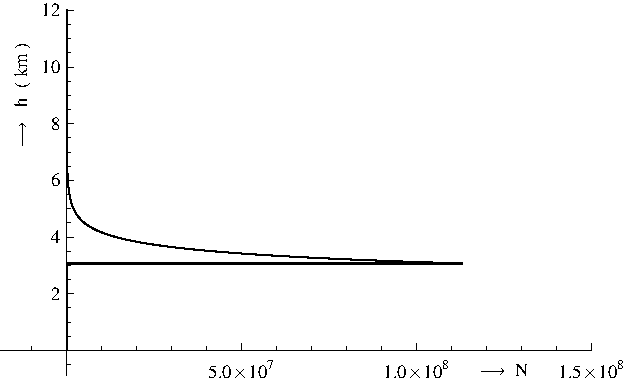
\includegraphics[width=12.0cm]{heitler.pdf}
    \caption{Het aantal elektronen en positronen in een shower volgens
             het Heitler model (horizontaal) als functie van de hoogte
             (vertikaal).}
    \label{fig:heitler}
\end{figure}

In werkelijkheid wordt bij een splitsing de energie niet gelijk
verdeeld. Ook duurt het bij het ene deeltje langer voor het splitst dan
bij het andere deeltje; dat hangt van het toeval af. Het belangrijkste
gevolg is dat de shower niet plotseling stopt, maar geleidelijk afneemt
(\figref{fig:greisen}).

\begin{figure}
    \centering
    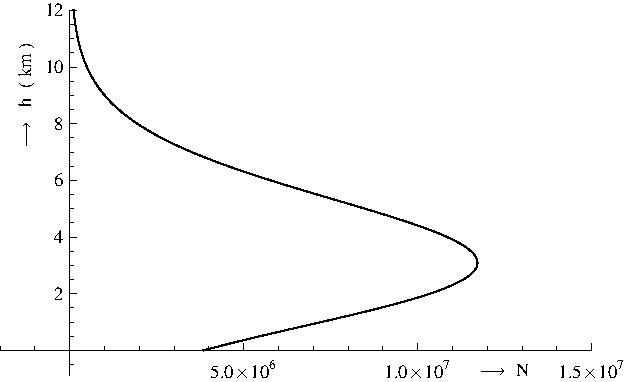
\includegraphics[width=12.0cm]{greisen.pdf}
    \caption{Het aantal elektronen en positronen in een shower volgens
             een realistisch model (horizontaal) als functie van de
             hoogte (vertikaal).}
    \label{fig:greisen}
\end{figure}

We zien duidelijk dat de ontwikkeling van de shower volgens het Heitler
model veel verschilt van de werkelijkheid. Het maximum aantal deeltjes
is volgens het Heitler model bijna 10 keer te groot. Dat er toch waarde
wordt gehecht aan het Heitler model komt omdat het de hoogte waarop het
maximum aantal deeltjes wordt bereikt wél goed voorspelt. Voor de
voorbeeld shower van \SI{8}{\peta\electronvolt} is die hoogte ongeveer
\SI{3}{\km}. Verder zien we dat volgens het Heitler model de shower op
\SI{3}{\km} hoogte ophoudt, terwijl in werkelijkheid voor de voorbeeld
shower van \SI{8}{\peta\electronvolt} er ongeveer 4 miljoen elektronen
en positronen het aardoppervlak bereiken. Als die een signaal afgeven in
een \hisparc detector wordt de shower geregistreerd.


\subsection{Hadronische showers}

Wanneer een kosmisch proton $p$ de dampkring binnenkomt, kan het een
sterke (hadronische) wisselwerking aangaan met de kern van een
luchtatoom. Het gevolg is dat er een groot aantal pionen ontstaat.
Daarvan is ongeveer een derde deel positief geladen ($\pi^+$), een
derde deel negatief geladen ($\pi^-$) en  een derde deel ongeladen
(neutraal) ($\pi^0$). De neutrale pionen hebben een extreem korte
levensduur; ongeveer \SI{8,4e-17}{\second} in rust. Ze vervallen daardoor
direct in twee gamma-deeltjes die elk een elektromagnetische shower
teweegbrengen zoals hiervoor beschreven. De geladen pionen hebben een
langere levensduur; ongeveer \SI{2,6e-8}{\second} in rust. De hoge snelheid
van de geladen pionen veroorzaakt tijddilatatie (een gevolg van de
relativiteitstheorie) waardoor de levensduur veel groter is. Het gevolg
is dat de geladen pionen een sterke wisselwerking aangaan met de kern
van een luchtatoom voor dat hun levensduur voorbij is. Daarbij ontstaan
weer nieuwe pionen, waarvan weer een derde deel $\pi^+$, een derde
deel $\pi^-$ en een derde $\pi^0$. De neutrale pionen daarvan
vervallen weer direct tot twee gamma deeeltjes, terwijl de geladen
pionen weer een sterke wisselwerking aan kunnen gaan, enzovoort. Na een
aantal sterke wisselwerkingen is de energie van per pion, en daarmee ook
zijn levensduur, zodanig afgenomen dat het pion vervalt voordat het een
sterke wisselwerking aangaat. Het geladen pion vervalt dan in een muon
$\mu$ (met dezelfde lading als het pion) en een muonneutrino $\nu_\mu$
(ongeladen). In een schema:
\begin{equation}
    \pi^+ \rightarrow \mu^+ + \nu_\mu \ , \nonumber
\end{equation}
\begin{equation}
    \pi^- \rightarrow \mu^- + \bar{\nu}_\mu \ , \nonumber
\end{equation}
\begin{equation}  
    \pi^0 \rightarrow \gamma + \gamma \ . \nonumber
\end{equation}

Net als de pionen hebben de muonen ook een eindige levensduur; ongeveer
$2,2 \cdot 10^{-6}$ s in rust. De muonen die in de hadronische shower
ontstaan hebben een dusdanige hoge energie (en daarmee een dusdanige
levensduur) dat ze veelal het aardoppervlak bereiken. Omdat ze geladen
zijn kunnen ze net als de elektronen een signaal afgeven in de \hisparc
detector. De muonen die niet het aardoppervlak bereiken zijn ergens in
de lucht vervallen in een elektron en twee verschillende neutrino's:
\begin{equation}
    \mu^+ \rightarrow e^+ + \nu_e + \bar{\nu}_\mu \ , \nonumber
\end{equation}
\begin{equation}
    \mu^- \rightarrow e^- + \bar{\nu}_e + \nu_\mu \ . \nonumber
\end{equation}  

Sommige elektronen (positronen) die ontstaan zijn uit het verval van
muonen kunnen alsnog het aardoppervlak bereiken en een signaal afgeven
in een \hisparc detector.
\\

De hadronische shower is belangrijk omdat bijna 90\% van de kosmische
deeltjes protonen zijn.
 

\section{Levensduur en relativiteit}

Eerder kwam al de verlenging van de levensduur van een energetisch
deeltje ter sprake. Volgens de relativiteitstheorie geldt voor de
levensduur van een bewegend deeltje:
\begin{equation}
    \tau (v) = \frac{\tau^0}{\sqrt{1-\frac{v^2}{c^2}}} \ . \nonumber
\end{equation}

Hierin is $v$ de snelheid van het deeltje en $c$ de lichtsnelheid.
Verder is $\tau^0$ de levensduur van een deeltje in rust. Als een muon
een snelheid heeft dat 99,9\% is van de lichtsnelheid, dan is zijn
levensduur 
\begin{equation}
    \tau(0,999c) = \frac{\tau^0}{\sqrt{1-0,999^2}}
    = \frac{2,2 \cdot 10^{-6}}{\sqrt{1-0,999^2}}
    = 4,9 \cdot 10^{-5} \SI{}{\second}. \nonumber
\end{equation}
Voor de afstand $x$ die dit muon aflegt voor het vervalt vinden we dan 
\begin{equation}
    x = v \cdot \tau (v)
    = 0,999c \cdot \tau (0,999c)
    = 0,999 \cdot 3 \cdot 10^8 \cdot 4,9 \cdot 10^{-5}
    = 1,47 \cdot 10^4 \SI{}{\meter}. \nonumber
\end{equation}
Dat is bijna \SI{15}{\km}. 
\\

Tot slot moet worden benadrukt dat de levensduur eigenlijk een
\textbf{gemiddelde} levensduur betreft. Als er wordt gezegd dat de
levensduur van bijvoorbeeld een geladen pion in rust
\SI{2,6e-8}{\second} is, dan is die waarde een verwachtingswaarde. Een
individueel pion kan best korter of langer leven, maar gemiddeld over
een groot aantal pionen klopt het. Dit geldt voor alle deeltjes met
eindige levensduur.


\begin{thebibliography}{9}
    \bibitem{strang} Foto door U.S. Air Force Senior Airman J. Strang.
\end{thebibliography}


\end{document}
